\subsection{Voltage}
\label{sec:results_voltage}

These are our results when measuring voltage with our multimeter. The tests were performed with a power supply sweeping the voltage from 0 to 20V. While this was happening the voltage was measured by our multimeter and a calibrated one. The test has been performed with the use of Keysight 34461A Digital Multimeters which is referred to as Calibrated.

\begin{figure}[h]
    \centering

    \begin{tikzpicture}

    \begin{axis}[legend style={at={(0.95, 0.1)},anchor=south east}, width=\linewidth, height=5cm,
        title = {Voltage Measurement},
        xlabel = {Target [V]},
        ylabel = {Measured [V]}]
        \addplot[blue, mark=*] table {Results/VoltData/VoltageMeasCal.dat};
        \addlegendentry{Calibrated}
        \addplot[red, mark=*] table {Results/VoltData/VoltageMeasOur.dat};
        \addlegendentry{Voltmeter}
    \end{axis}

    \end{tikzpicture}

    \caption{The measured voltage by both calibrated and our multimeters from what target was set.}
    \label{fig:ResVoltageMeas}
    
\end{figure}
% \begin{figure}[h]
%     \centering
%     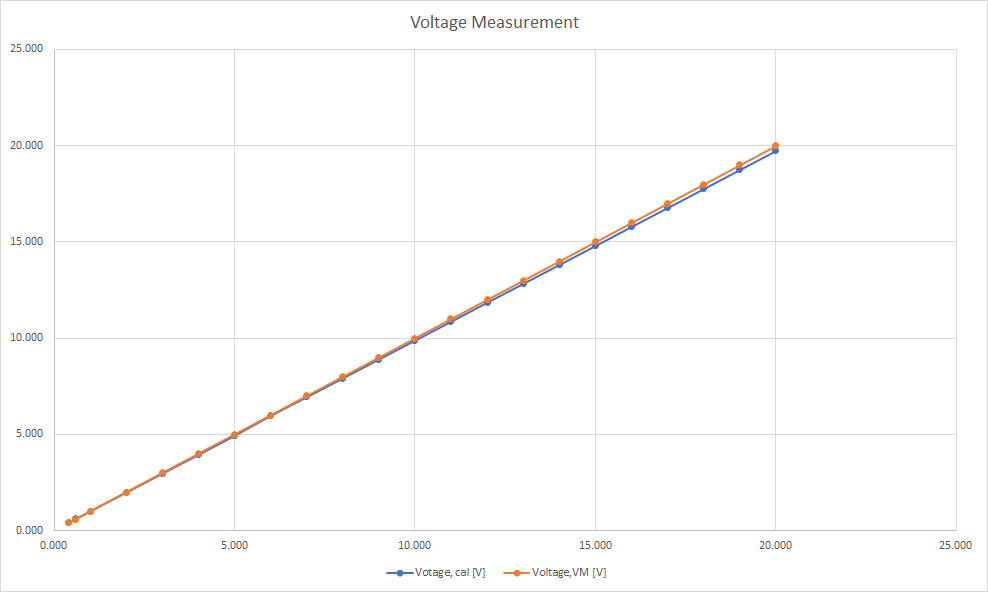
\includegraphics[width=0.80\linewidth]{images/voltageMeas.png}
%     \caption{Voltage Measurements}
%     \label{fig:ResVoltageMeas}
% \end{figure}
Figure \ref{fig:ResVoltageMeas} shows the voltage measured by a power supply internal meter, the calibrated one as well as ours.

\begin{figure}[h]
    \centering

    \begin{tikzpicture}

    \begin{axis}[legend style={at={(0.95, 0.4)},anchor=south east}, width=\linewidth, height=5cm,
        title = {Percentage deviation, voltage},
        xlabel = {Target [V]},
        ylabel = {Percentage [\%]}]
        \addplot[red, mark=*] table {Results/VoltData/VoltageDeltaCal.dat};
    \end{axis}

    \end{tikzpicture}

    \caption{The difference from the target or the measured value by the calibrated multimeter at different target settings.}
    \label{fig:ResVoltageDelta}
    
\end{figure}
% \begin{figure}[h]
%     \centering
%     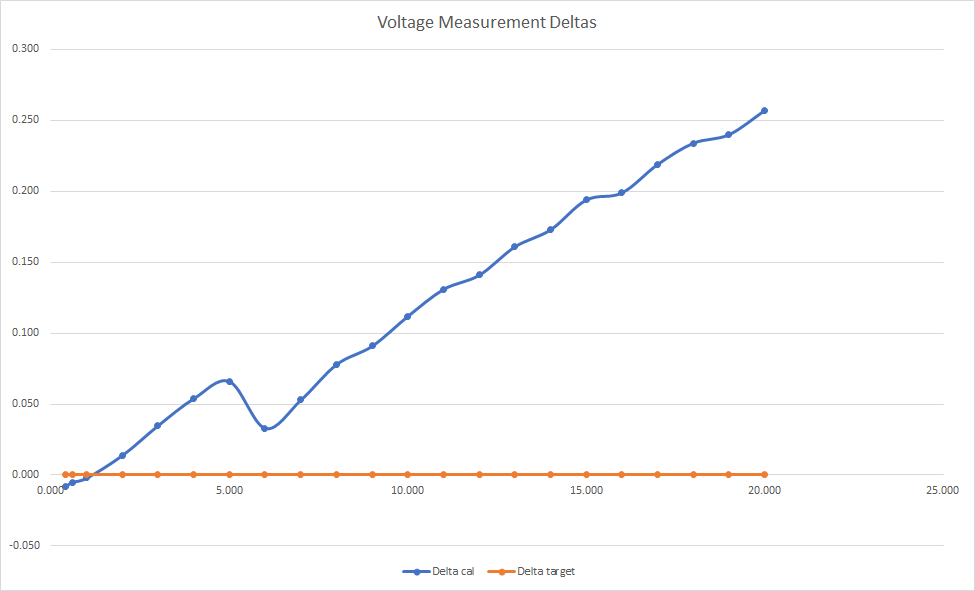
\includegraphics[width=0.80\linewidth]{images/voltageDelta.png}
%     \caption{Voltage Deltas}
%     \label{fig:ResVoltageDelta}
% \end{figure}
Figure \ref{fig:ResVoltageDelta} shows the difference between our multimeter measurement and the measurement of the calibrated one as well as the set point on the power supply. See Figure \ref{fig:VM1} for test setup.
